
\begin{figure}
\begin{minipage}[height=.05\textheight]{.5\textwidth}
\centering
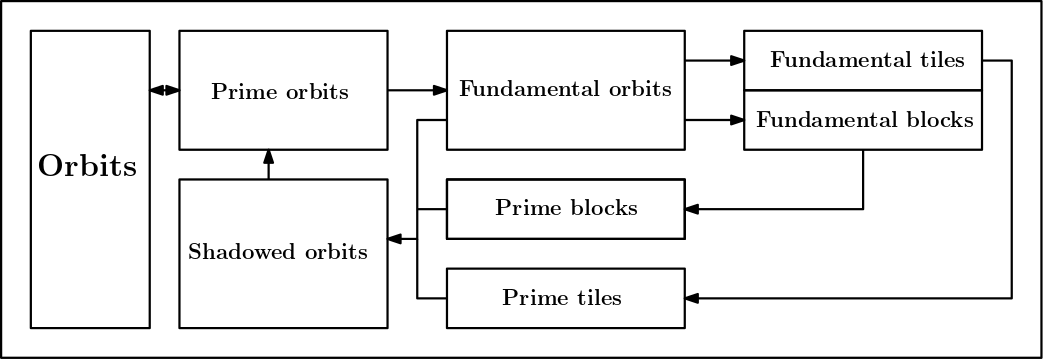
\includegraphics[width=.8\textwidth,height=.2\textheight]{MNG_orbitblocktile_flow_chart}
\end{minipage}
\caption{ \label{fig:MNG_flowchart}
This flow chart represents the order that is required to make
{\spt} constructions. The flow from orbits to prime orbits to fundamental
orbits represents the process of searching for solutions and then clipping
out the fundamental tiles. Once the fundamental tiles are converged, the
fundamental tiles are well defined (the space-time on which the fundamental
orbit sits) as well as the fundamental blocks (the names that we assign
to the unique pattern found in the fundamental orbit). In order to glue,
there are three requirements, the prime configuration of blocks, the
prime tile that they are defined on, and the
approximate state that exists on the prime tile. Only after the prime
tile and prime block are in place can the fundamental orbits be
laid out on the prime tile. With this, an approximate solution that is
shadowed by a prime orbit is made. By converging this shadowed orbit
we arrive at the prime orbit it is shadowed by. Symmetry operations and
space-time periodicity then produce the entire (global) orbit.
}
\end{figure}